% 第3章按课件顺序重写；本章课件 PDF 页码与幻灯片显示页码相同。
\chapter{数据链路层与局域网}

\noindent 本章课件共 153 页，依次讲解数据链路层服务、差错检测与纠正、可靠数据传输、多路访问控制、局域网技术、PPP 和链路虚拟化。以下按课件的章节顺序整理。课件 PDF 页码与页面右下角显示页码相同；引用教材时同时标出 PDF 阅读器页与印刷页。

\section{数据链路层服务}

\subsection{数据链路层负责一段链路上的传输}
\textbf{结点（node）}是网络中的主机、路由器或交换机。\textbf{链路（link）}是连接相邻结点的通信信道，可以是有线链路、无线链路或局域网。这里的“相邻”指两个结点直接通过同一条链路通信。

数据链路层位于网络层和物理层之间：向下使用物理层提供的比特传输服务，向上向网络层提供明确的服务接口。它负责将网络层交下来的\textbf{数据报}封装成\textbf{帧（frame）}，并通过一条链路送到直接相连的下一结点。帧是第 2 层的协议数据单元，载荷通常是网络层数据报。

若主机 A 经路由器 R 向主机 B 发送数据，A--R 链路上的帧到达 R 后，R 取出其中的数据报；R 再将数据报封装为适合 R--B 链路的帧。数据报可跨越多条链路，帧则服务于当前一段链路。不同链路可以使用不同的帧格式。

局域网（Local Area Network，LAN）数据链路层常分为两个子层：\textbf{逻辑链路控制（Logical Link Control，LLC）}面向上层服务，\textbf{介质访问控制（Medium Access Control，MAC）}处理帧如何使用共享介质。课件图中的发送过程是“网络层数据报 → 数据链路层封装成帧 → 物理层发送比特”；接收过程按相反方向处理。

\annotationarea{4}

\subsection{组帧、帧同步与透明传输}
\textbf{组帧（framing）}是把网络层数据报封装为帧。\textbf{帧同步}是从物理层交付的连续比特流中识别每一帧的开始和结束。\textbf{透明传输}要求接收方还原出原始载荷，即使载荷本身含有与帧边界相同的字节或比特组合，也不能把数据误认成边界。

\paragraph{字节计数法。} 在帧首部放入帧长度或计数字段，接收方据此读出一帧。课件第 7 页的四帧示例分别标出 5、5、8、6 字节。若计数字段本身传错，例如把 5 读成 7，接收方就可能多读后续帧的两个字节，之后的边界也随之错位。因此，单独依赖计数字段容易因该字段出错而失去同步。

\paragraph{定界符与字节填充。} 用特殊字节 \texttt{FLAG}（例如 \texttt{0x7E}）表示边界。若载荷中也出现 \texttt{FLAG}，发送方在该字节前插入转义字节 \texttt{ESC}；载荷中的 \texttt{ESC} 自身也需转义。接收方在帧内部看到 \texttt{ESC} 时，将其后的字节还原为普通数据。
\begin{quote}\small
课件示意：原载荷 \texttt{A FLAG ESC B}；填充后为 \texttt{A ESC FLAG ESC ESC B}；线上帧在其前后再加边界 \texttt{FLAG}。接收方去掉两端边界，并按转义规则解码，恢复原载荷。
\end{quote}

\paragraph{定界符与比特填充。} 用比特串 \texttt{01111110} 表示帧边界。发送方只扫描帧内部的载荷，每出现连续 5 个 1 就插入一个 0；首尾的定界符不填充。接收方识别帧边界后，在帧内部每串连续 5 个 1 后删除发送方插入的 0。
\[
  \text{载荷 }01111110\quad\longrightarrow\quad
  \text{填充后 }011111010.
\]
原载荷的中间有连续 6 个 1；插入 0 后不再出现与定界符相同的连续 6 个 1。接收端删除填入的 0 后恢复原比特串。

\begin{figure}[H]
 \centering
 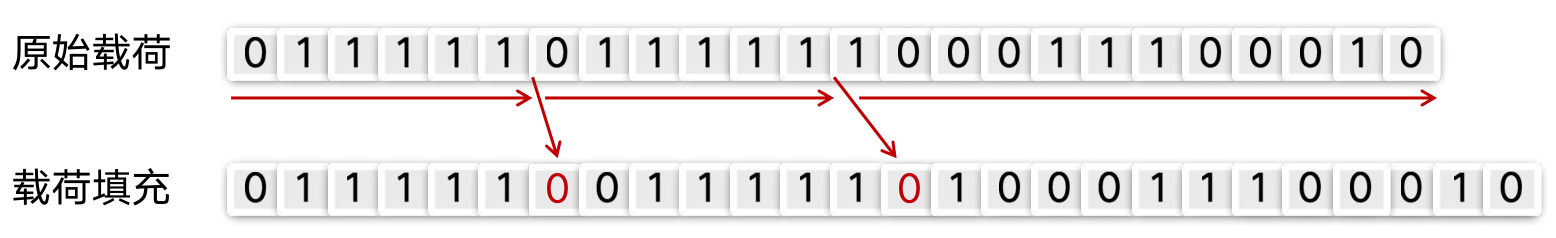
\includegraphics[width=0.82\textwidth]{ch03-bit-stuffing.png}
 \caption{帧内连续 5 个 1 后插入 0，接收时删除该 0。来源：\texttt{Chapter3-数据链路层.pdf}，PDF 第 11 页（显示页 11），局部截取。}
 \label{fig:ch03-bit-stuffing}
\end{figure}

\paragraph{物理层编码违例。} 若一种物理层编码有未使用的码字或信号模式，可把它用作边界。课件列举 4B/5B 编码中未使用的码字、传统以太网和 802.11 中的长前导码，以及曼彻斯特或差分曼彻斯特编码中比特周期中间无跳变的模式（课件以 802.5 令牌环为例）。该办法成立的前提是所选模式不会作为普通数据编码出现。

\annotationarea{4}

\subsection{链路层可能提供的其他服务}
数据链路层的功能不只组帧。不同协议会按需要提供下列服务，并非每种链路层协议都实现全部功能。

\begin{itemize}
 \item \textbf{物理寻址：}帧首部可以带有源和目的 MAC 地址，用于标识局域网内帧从哪个接口发出、交给哪个接口。MAC 地址的具体形式见“局域网技术”。
 \item \textbf{差错控制：}发送端可加入差错编码位，接收端检测帧是否损坏；某些编码可直接纠正错误，某些协议发现错误后请求重传，也有协议直接丢弃差错帧。
 \item \textbf{相邻结点间可靠交付：}通过确认、序号与重传等机制，处理损坏、丢失、乱序或重复。课件指出，无线链路误码率较高，常需要停等或滑动窗口机制；低误码率有线链路较少逐帧实现可靠传输。
 \item \textbf{流量控制：}协调相邻发送方与接收方的发送速度，避免接收端处理不过来或缓存耗尽。反馈式流量控制由接收方反馈状态，发送方据此调速；速率式流量控制由发送方按内建机制限速。
 \item \textbf{介质访问控制：}多个结点共用一个物理信道时，协调结点何时发送。
 \item \textbf{双工方式：}全双工允许链路两端同时双向传输；半双工允许双向通信，但两端交替发送。
 \item \textbf{服务类型：}无连接服务不先建立数据链路层连接；面向连接服务在交换数据前先建立连接。是否提供可靠交付是另一项独立属性。
\end{itemize}

\textbf{网卡（Network Interface Card，NIC）}或网络适配器实现数据链路层和物理层功能。它安装在主机或路由器的接口处，通过系统总线与主机相连，通常由控制器、硬件、固件和软件共同完成帧封装、比特发送、差错检测以及协议规定的流量控制和可靠传输。

\begin{quote}\small 来源：课件 PDF 第 3--16 页（显示页 3--16）；参考书 §3.1--§3.2，PDF 第 61--66 页（印刷第 50--55 页）。课件给出组帧、寻址、流量控制、差错控制、访问控制、半/全双工、连接服务和网卡实现等内容。\end{quote}
\annotationarea{4}

\section{差错检测与纠正}

\subsection{差错编码与汉明距离}
传输中的衰减和噪声可能导致比特翻转。发送方把原数据 $D$ 与若干\textbf{冗余比特} $R$ 组合成码字；接收方根据编码规则检查收到的码字。冗余位能提高检错或纠错能力，但任何有限编码都不能保证检测所有可能差错。

两个等长码字逐位比较时，不同位的个数称为\textbf{汉明距离}。例如，\texttt{0110} 与 \texttt{0011} 有两位不同，距离为 2。一个编码集合的最小汉明距离 $d_{\min}$，是所有不同合法码字之间距离的最小值。

课件给出的保证条件是：若 $d_{\min}=r+1$，可以检测任意不超过 $r$ 位的差错；若 $d_{\min}=2r+1$，可以纠正任意不超过 $r$ 位的差错。一般写成
\[
  \text{保证检出 }s\text{ 位错： }d_{\min}\ge s+1,\qquad
  \text{保证纠正 }t\text{ 位错： }d_{\min}\ge 2t+1.
\]
检错要求错误后的码字不落到另一个合法码字上；纠错还要求错误后的接收串离原码字比离其他合法码字更近。

\textbf{课件例题 1：检错码。} 编码集合为 $\{0000,0101,1010,1111\}$。任意两个不同码字至少有 2 位不同，因此 $d_{\min}=2$，能保证检测 1 位差错，但不能保证纠正 1 位差错。

\textbf{课件例题 2：纠错码。} 编码集合为 $\{000000,010101,101010,111111\}$，最小距离为 3，能保证纠正 1 位差错。若收到 \texttt{100010}，它与合法码字 \texttt{101010} 只差 1 位，因此在“最多 1 位差错”的前提下纠正为 \texttt{101010}。

\annotationarea{4}

\subsection{奇偶校验}
\textbf{一维奇偶校验}在数据后增加一个校验位，使码字中 1 的总数为偶数（偶校验）或奇数（奇校验）。若采用偶校验，任意奇数个比特翻转会改变 1 的个数奇偶性，因而可检测；偶数个比特翻转可能保持奇偶性，不能保证检测。一个校验位不能指出出错位置。

\textbf{二维奇偶校验}将数据位排成行和列，分别计算行、列校验位。若只有一个数据位翻转，会有且只有一行、 一列校验失败；行列交点就是错误位，可以据此纠正。多个错误可能使部分或全部行列校验再次满足，故不应把单比特定位的结论扩大到任意多比特错误。课件第 20 页将可纠错情形作了简写，使用时须带上“只有一个错误位”的条件。

\annotationarea{4}

\subsection{Internet 校验和}
Internet 校验和用于 IP、TCP、UDP 等协议的差错检测。发送方把待检内容按 16 位分组；最后不足 16 位的部分按规则补零。对各 16 位字进行反码加法：最高位产生的进位 1 回卷并加到最低位，若仍有进位则继续回卷。将最终和逐位取反，得到校验和并填入校验和字段。

接收端对收到的数据和校验和执行相同的 16 位反码加法。若数据与校验和相加为 16 个 1（再取反为全 0），检查通过；否则检出差错。检查通过只表示没有检出差错，并不保证传输绝对无错。

\annotationarea{4}

\subsection{循环冗余校验 CRC}
\textbf{循环冗余校验（Cyclic Redundancy Check，CRC）}使用模 2 除法生成检错位。模 2 加减法就是逐位异或 $\oplus$，不产生进位或借位，例如 $1\oplus1=0$、$1\oplus0=1$。

发送端与接收端预先约定生成比特串 $G$。若 $G$ 长度为 $r+1$ 位，则其对应多项式次数为 $r$。发送端在数据串 $D$ 后附加 $r$ 个 0，得到 $D\cdot 2^r$；用 $G$ 对其作模 2 长除，所得余数 $R$ 长度不超过 $r$ 位，必要时在左侧补 0 至 $r$ 位。发送的码字为 $D$ 后接 $R$。接收端用同一个 $G$ 除收到的完整码字：余数全 0 表示未检出差错，非零表示检出差错。

\textbf{课件例题（PDF p.23）。} 数据 $D=101110$，生成串 $G=1001$，因此 $r=3$，先补 3 个 0：
\[
 D\cdot 2^r=101110000.
\]
模 2 长除按每一步对齐最高位的 1 后异或：
\begin{center}
\begin{tabular}{c c}
\toprule
当前被除串 & 本步异或后的串\\
\midrule
\texttt{101110000} $\oplus$ \texttt{100100000} & \texttt{001010000}\\
\texttt{001010000} $\oplus$ \texttt{001001000} & \texttt{000011000}\\
\texttt{000011000} $\oplus$ \texttt{000010010} & \texttt{000001010}\\
\texttt{000001010} $\oplus$ \texttt{000001001} & \texttt{000000011}\\
\bottomrule
\end{tabular}
\end{center}
最后的余数为 3 位 $R=011$，所以发送 \texttt{101110011}。将其再除以 \texttt{1001}，余数为 \texttt{000}。

CRC 常用于帧的差错检测。课件指出，次数为 $r$ 的生成多项式能检测所有长度小于 $r+1$（即不超过 $r$）位的突发差错。\textbf{突发差错长度}从第一个错误位到最后一个错误位计数，中间即使有正确位也计入长度。更长突发错误通常也能检测，但不能保证全部检出。

\annotationarea{4}

\subsection{检错之后的处理}
差错处理有不同方案：\textbf{前向纠错（Forward Error Correction，FEC）}使用纠错码，让接收端在编码保证范围内直接修正比特；\textbf{检错重传}发现损坏后通过停等或滑动窗口协议请求再次发送；\textbf{检错丢弃}发现错误就丢弃帧；\textbf{反馈校验}将校验信息反馈给发送端。CRC 主要用于检错，不能单独恢复丢失帧。

\begin{quote}\small 来源：课件 PDF 第 17--24 页（显示页 17--24）；参考书 §3.3，PDF 第 67--71 页（印刷第 56--60 页）。CRC 例题采用课件第 23 页的 $D=101110$、$G=1001$；课件第 20 页二维奇偶校验的纠错能力按单比特差错条件表述。\end{quote}
\annotationarea{4}

\section{可靠数据传输}

\subsection{可靠传输的目标和协议接口}
可靠传输要求数据\textbf{不错、不丢、不乱、不多}：内容正确，没有缺失，按顺序交付，不重复交付。网络层、传输层和链路层都可能需要可靠传输机制。课件先用单向数据传输作为讲解模型，但确认等控制信息会沿反方向传送。

课件使用以下接口描述协议动作：\texttt{rdt\_send()} 表示上层交数据给可靠传输协议；\texttt{udt\_send()} 表示可靠传输协议把分组交给不可靠信道；\texttt{rdt\_rcv()} 表示分组到达接收方；\texttt{deliver\_data()} 表示接收方将数据交给上层。有限状态机（Finite State Machine，FSM）用状态记录协议正在等待什么；外部事件触发状态转移，并执行相应动作。

\annotationarea{4}

\subsection{rdt 1.0、2.0、2.1、2.2 与 3.0}
\textbf{rdt 1.0：可靠信道。} 假定底层信道不会出错也不会丢失分组。发送方收到上层数据后封装并发送；接收方收到后取出数据交给上层，不需要确认或重传。

\textbf{rdt 2.0：可能发生比特错误。} 发送方加入校验和；接收方正确收到后回送肯定确认（Acknowledgment，ACK），发现损坏后回送否定确认（Negative Acknowledgment，NAK）；发送方收到 NAK 后重传。基于反馈与重传的协议称为自动重传请求（Automatic Repeat reQuest，ARQ）。rdt 2.0 每次只发送一个分组并等待反馈，属于停等。其缺陷是 ACK/NAK 本身也可能损坏；发送方无法判断接收方是否已经收下数据，若直接重发便可能造成重复交付。

\textbf{rdt 2.1：使用序号识别重复分组。} 发送方交替使用序号 0 和 1。新分组使用下一个序号；同一分组重传时保留原序号。接收方记住期望序号：收到正确且期望的分组才交付一次并切换期望值；收到重复旧分组时不再次交付，但重新发送确认。此时假设分组不会完全丢失。

\textbf{课件思考：为什么 0 和 1 两个序号就够？} 停等时，发送方任一时刻最多有一个未确认的数据分组。接收方只需区分当前期望的新分组与上一个已接收分组的重传，因此 1 位序号（0、1 交替）即可。收到相同旧序号时，接收方知道是重复副本。

\textbf{rdt 2.2：不使用 NAK。} 接收方只发送 ACK，并在 ACK 中标明所确认分组的序号。若收到损坏或非期望分组，接收方再次确认最后一个正确收到的分组。发送方收到重复 ACK 时执行与 NAK 相同的动作，即重传当前分组。

\textbf{rdt 3.0：还可能发生分组丢失。} 发送方发送分组后启动计时器；收到正确且序号匹配的 ACK 后停止计时器。超过等待时间仍未收到 ACK，就重传原分组并重新计时。数据分组或 ACK 若只是延迟，重传可能产生重复分组，仍由序号机制识别。

\annotationarea{4}

\subsection{rdt 3.0 事件例题：无损、数据丢失与确认丢失}
课件 PDF 第 44--45 页用四条时间线说明停等协议。下表中的“交付”指接收方交给上层；“重复”指同一序号的旧副本。

\begin{enumerate}
 \item \textbf{无损：}发送方发送 pkt0；接收方收到并交付 pkt0，回 ACK0；发送方收到 ACK0 后发送 pkt1；接收方交付 pkt1 并回 ACK1。双方按序号交替继续。
 \item \textbf{数据分组丢失：}发送方发 pkt1，但该分组丢失；等待超时后仍用序号 1 重发 pkt1；接收方首次收到 pkt1 后交付并回 ACK1。
 \item \textbf{ACK 丢失：}接收方收到 pkt1 并交付，发出的 ACK1 丢失；发送方超时后重发 pkt1；接收方发现 pkt1 是重复副本，不再次交付，再回 ACK1；发送方收到后停止计时并可发送下一新分组。
 \item \textbf{过早超时：}发送方的计时器先于延迟的 ACK1 到期，于是重发 pkt1；接收方识别重复分组并再次回 ACK1。发送方收到一份匹配的 ACK1 后可继续；之后到达的重复 ACK 因序号不匹配当前状态而被忽略。
\end{enumerate}

\textbf{做题要点：}超时只说明发送方尚未得到确认，不能断定一定是数据分组丢失；可能丢的是 ACK，也可能只是延迟。接收方的序号检查负责去重，计时器负责打破无限等待。

\begin{figure}[H]
 \centering
 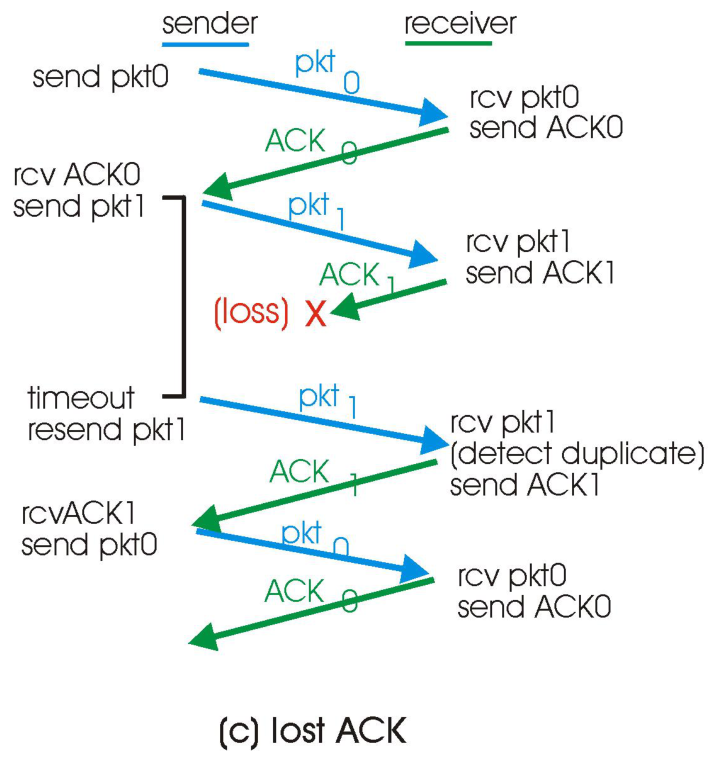
\includegraphics[width=0.9\textwidth]{ch03-ack-loss-detail.png}
 \caption{ACK 丢失后重传相同序号的分组，接收端识别重复并再次确认。时间向下，箭头表示分组或 ACK。来源：\texttt{Chapter3-数据链路层.pdf}，PDF 第 45 页（显示页 45），局部截取。}
 \label{fig:ch03-ack-loss}
\end{figure}

\annotationarea{4}

\subsection{停等协议的信道利用率}
设数据分组长 $L$ bit，发送速率 $R$ bit/s，则发送一个数据分组的时间为 $t_{\mathrm{seg}}=L/R$。确认分组长 $L_{\mathrm{ACK}}$ bit、反向链路速率 $R_{\mathrm{ACK}}$ bit/s，则确认发送时间 $t_{\mathrm{ACK}}=L_{\mathrm{ACK}}/R_{\mathrm{ACK}}$。\textbf{往返时间（Round-Trip Time，RTT）}按课件时间图理解：从数据分组最后一位发出，到 ACK 第一位返回发送端的往返等待时间；ACK 完整到达还需 $t_{\mathrm{ACK}}$。

从发送一帧开始到完整收到 ACK，一个停等周期为 $t_{\mathrm{seg}}+\mathrm{RTT}+t_{\mathrm{ACK}}$。无差错且收到确认后立即发送下一帧时，链路用于发送数据帧的比例为
\[
 U_{\mathrm{stop}}=
 \frac{t_{\mathrm{seg}}}{t_{\mathrm{seg}}+\mathrm{RTT}+t_{\mathrm{ACK}}}.
\]
它是发送端等待期间的时间利用率，不是载荷占帧长的比例。计算时须按题目给出的 RTT 定义，避免重复计算已经包含的时间。

\textbf{课件例题（PDF p.46--48）。} 链路速率为 $1\,\mathrm{Gb/s}$，单程传播延迟 $15\,\mathrm{ms}$，每个分组长 $1\,\mathrm{KB}=8000$ bit。忽略 ACK 发送时间，则
\[
 t_{\mathrm{seg}}=\frac{8000}{10^9}\,\mathrm{s}=8\,\mu\mathrm{s},\qquad
 \mathrm{RTT}=2\times15\,\mathrm{ms}=30\,\mathrm{ms},
\]
\[
 U\approx\frac{8\,\mu\mathrm{s}}{8\,\mu\mathrm{s}+30\,\mathrm{ms}}
 =0.0002666\approx0.0267\%.
\]
有效发送速率约为 $1\,\mathrm{Gb/s}\times U=267\,\mathrm{kb/s}$，即约 $33\,\mathrm{kB/s}$。物理线路很快，但停等发送方的大部分时间在等 ACK。

\annotationarea{4}

\subsection{流水线和滑动窗口}
\textbf{流水线}允许发送方在收到确认前连续发送多个分组，可以减少线路空闲时间，但要求序号空间更大，并在发送方、接收方或两端缓存尚未确认的分组。\textbf{窗口}是当前允许使用的一段序号范围；窗口尺寸为 $N$ 时，最多可有 $N$ 个分组等待确认。随着确认到达，窗口沿序号空间向前滑动。

\begin{figure}[H]
 \centering
 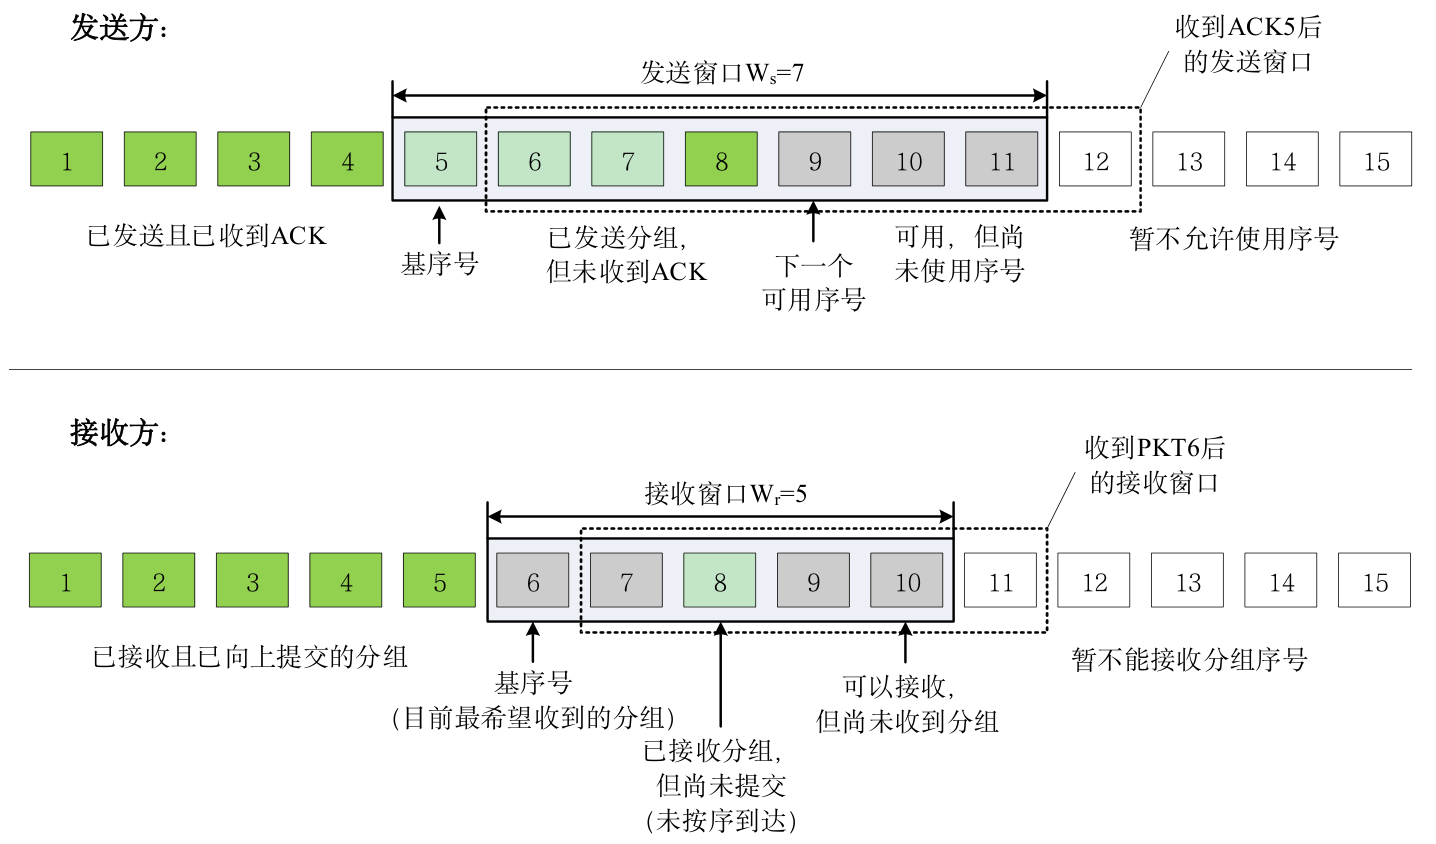
\includegraphics[width=0.88\textwidth]{ch03-sliding-window.png}
 \caption{发送窗口限制未确认分组；接收窗口限制可接收序号，窗口随确认或按序交付前移。来源：\texttt{Chapter3-数据链路层.pdf}，PDF 第 53 页（显示页 53），局部截取。}
 \label{fig:ch03-window}
\end{figure}

若序号字段有 $k$ bit，序号按模 $2^k$ 循环。课件给出的窗口约束为
\[
 W_s+W_r\le 2^k,
\]
其中 $W_s$ 是发送窗口尺寸，$W_r$ 是接收窗口尺寸。具体协议还需满足自己的限制：GBN 中 $W_r=1$，故 $W_s\le2^k-1$；典型 SR 取 $W_s=W_r=W$，因此 $W\le2^{k-1}$；停等取 $W_s=W_r=1$，至少需 $k=1$。

\textbf{课件思考：窗口大小影响什么？} 窗口增大后，允许同时有更多未确认分组，信道利用率和吞吐率可以提高；但发送和接收端要缓存更多分组，窗口还受序号空间、接收缓存、流量控制与拥塞控制条件限制。窗口并非越大越好，必须满足序号空间和接收能力的约束。

\annotationarea{4}

\subsection{后退 N 帧协议 GBN}
\textbf{后退 N 帧（Go-Back-N，GBN）}采用发送窗口 $W_s$ 和接收窗口 $W_r=1$。发送方可连续发送窗口内多个分组；接收方只接收当前期望的序号，乱序分组直接丢弃。

GBN 使用\textbf{累积确认}：ACK($n$) 表示按发送顺序截至序号 $n$（包含 $n$）的分组均已正确接收；序号回绕时按序号空间中的先后次序理解，而不是按普通整数大小比较。发送方可为最早未确认的分组设置计时器；该分组超时后，重传它以及之后所有已经发出但仍未确认的分组。接收方若收到乱序分组，会再次确认最近按序接收的分组。

\textbf{课件示例（PDF p.59）。} pkt2 在传输中丢失。接收方收到 pkt0、pkt1 后依次确认；pkt3、pkt4、pkt5 因不等于当前期望的 pkt2 而被丢弃，并重复确认 pkt1。发送方收到 ACK0、ACK1 后可继续发 pkt4、pkt5；pkt2 超时后，按 GBN 规则依次重发 pkt2、pkt3、pkt4、pkt5。接收方此后按序收到并交付这些分组。

\textbf{课件例题（PDF p.60）。} 发送方已经发送 0--7 号帧；计时器超时时只收到 0、2、3 号帧的确认。需要重发多少帧，分别是哪几帧？

\textbf{解：}GBN 确认是累积确认。最高连续确认到 3 号，因此 4、5、6、7 号帧尚未得到确认；超时后需要重发 4 帧，即 4、5、6、7 号帧。

\annotationarea{4}

\subsection{选择重传协议 SR}
\textbf{选择重传（Selective Repeat，SR）}对每个正确收到的分组分别确认。接收方把窗口内到达的乱序分组暂存，等缺少的较早分组到达后，再按序将连续分组交给上层。发送方只重传未确认的分组，并为每个未确认分组单独设置计时器。

\textbf{课件示例（PDF p.65）。} 发送窗口、接收窗口均为 4。发送 pkt0、pkt1 后，pkt2 丢失，pkt3 仍可发送。接收方收到 pkt0、pkt1，分别交付并回 ACK0、ACK1；pkt3 在接收窗口内但乱序到达，于是缓存并回 ACK3。发送方收到 ACK0 后发 pkt4，收到 ACK1 后发 pkt5；接收方将 pkt4、pkt5 缓存并分别确认。pkt2 超时，发送方只重发 pkt2。接收方收到 pkt2 后，连续交付缓存中的 pkt2、pkt3、pkt4、pkt5，接收窗口前移。

\textbf{窗口与序号的歧义例（课件 PDF p.66--67）。} 若序号只有 2 bit，则序号为 0、1、2、3。SR 的发送和接收窗口若都为 3，就有 $W_s+W_r=6>4$。接收窗口滑动后可能同时包含序号 0；此时收到 0，接收方无法只凭序号判断它是上一轮迟到的旧副本，还是新一轮的 0 号分组。故典型等大窗口必须满足 $W\le2^{k-1}$；$k=2$ 时最大窗口为 2。

\textbf{课件思考：SR 还能怎样设计？} 可以改变确认和缓存的实现细节，但任何变体都必须规定每个分组如何确认、乱序数据如何暂存和按序交付，并保证新旧序号不会发生歧义。课件给出的 SR 是本章采用的典型设计。

\begin{figure}[H]
 \centering
 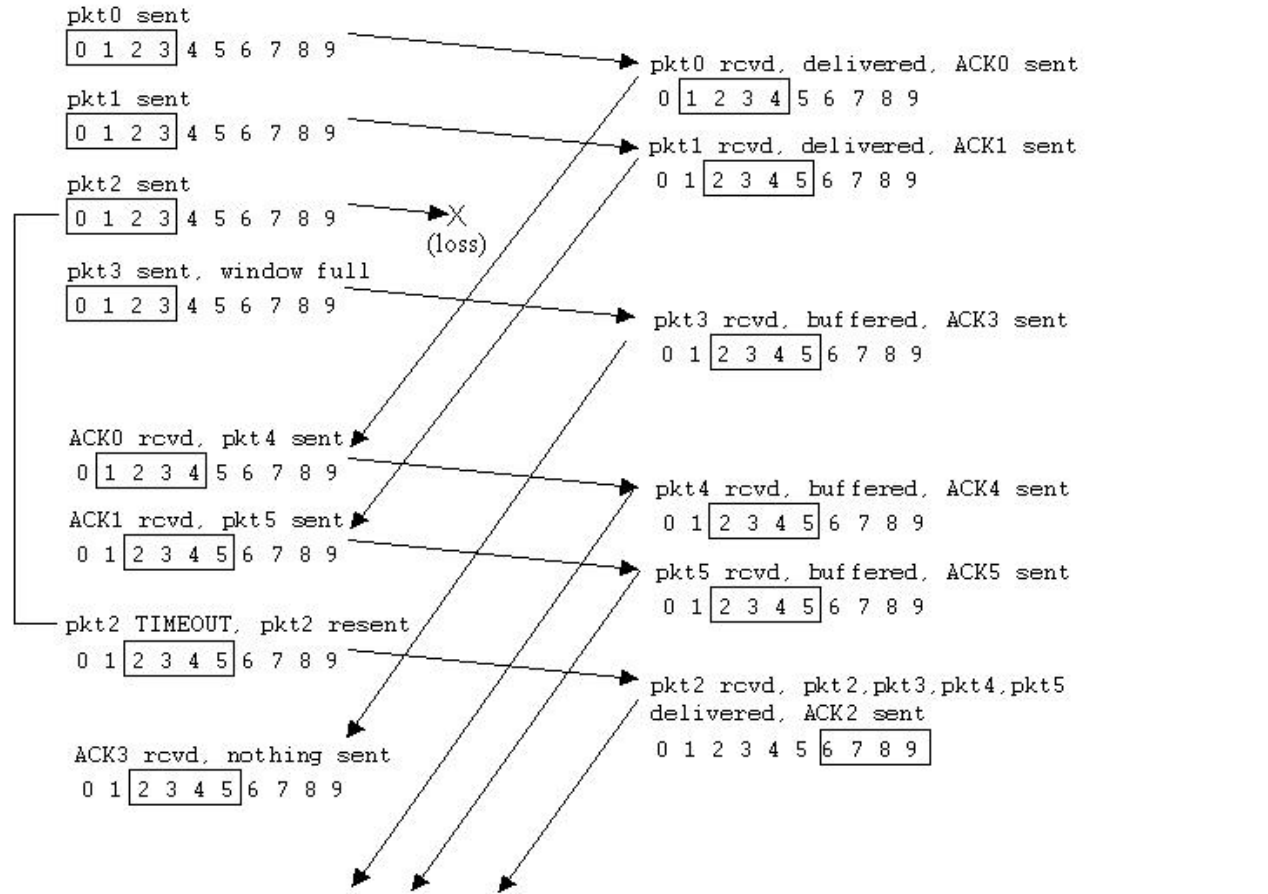
\includegraphics[width=0.98\textwidth]{ch03-sr-run-detail.png}
 \caption{SR 对 pkt0、pkt1、pkt3 等逐个确认并缓存乱序分组；pkt2 重传到达后按序交付缓存分组。来源：\texttt{Chapter3-数据链路层.pdf}，PDF 第 65 页（显示页 65），局部截取。}
 \label{fig:ch03-sr-run}
\end{figure}

\annotationarea{4}

\subsection{滑动窗口的利用率}
设连续发送窗口可容纳 $W_s$ 个分组，每个分组发送时间为 $t_{\mathrm{seg}}$，RTT 和 ACK 发送时间与停等定义相同。在无差错且发送端始终有数据时，窗口提供的理论利用率为
\[
 U=\min\!\left(1,\frac{W_s\,t_{\mathrm{seg}}}
 {t_{\mathrm{seg}}+\mathrm{RTT}+t_{\mathrm{ACK}}}\right).
\]
若 $W_s t_{\mathrm{seg}}$ 不足以覆盖一个确认往返周期，窗口耗尽后发送方仍需等待；当窗口能覆盖整个周期时，发送端可持续发送，利用率达到 1。实际吞吐还会受差错、重传、接收能力和可用带宽影响。

\begin{quote}\small 来源：课件 PDF 第 25--68 页（显示页 25--68）；参考书 §3.4，PDF 第 72--87 页（印刷第 61--76 页）。课件例题与事件图：rdt 3.0 第 44--45 页，停等性能第 46--48 页，GBN 第 59--60 页，SR 第 65--67 页。窗口上限按课件第 67 页所列约束表述。\end{quote}
\annotationarea{4}

\section{多路访问控制协议}

\subsection{共享广播信道和理想 MAC}
\textbf{点对点链路}只有两个通信端，例如拨号 PPP 或主机与交换机之间的专用链路。\textbf{广播链路}由多个结点共享，例如早期总线以太网、802.11 无线局域网。两个或更多结点同时在同一共享信道上传输，信号会相互干扰并发生\textbf{冲突（collision）}，接收失败。

\textbf{多路访问控制（MAC）协议}以分布式规则决定共享信道上的结点何时传输；协调信息也通过共享信道传送，没有另设带外协调信道。理想 MAC 希望：只有一个结点发送时可用全部速率 $R$；有 $M$ 个结点发送时平均每个结点获得 $R/M$；不依赖特定中心结点和同步时钟，并且规则简单。

课件将 MAC 协议分为三类：\textbf{信道划分}（预先分配时间、频率或编码资源）、\textbf{随机访问}（允许竞争与冲突，再通过规则恢复）、\textbf{轮转访问}（按顺序把发送机会交给结点）。

三类机制在不同负载下的取舍不同：信道划分在负载重时可稳定、公平地分享信道，但负载轻时未使用的预留资源会空闲；随机访问在负载轻时，单个结点可使用整个信道速率，负载重时冲突开销增加；轮转访问试图综合两者的优点。

\annotationarea{4}

\subsection{信道划分：TDMA、FDMA、CDMA 和 WDMA}
\textbf{时分多路访问（Time Division Multiple Access，TDMA）}把时间按周期分成固定时隙，每个站每周期使用指定时隙。若站点没有数据，其时隙仍空闲。课件例子中 6 个站点各有一个时隙，只有站点 1、3、4 发送，站点 2、5、6 的时隙未用。

\textbf{频分多路访问（Frequency Division Multiple Access，FDMA）}把信道频谱分成若干频带，每个站使用固定频带。无数据的站所分频带空闲。与 TDMA 不同，多个频带可在同一时刻同时传输。

课件还列出\textbf{码分多路访问（Code Division Multiple Access，CDMA）}和\textbf{波分多路访问（Wavelength Division Multiple Access，WDMA）}。CDMA 用不同码片序列区分同一信道上的信号；参考书补充说明，发送端用自己的码片表示 1、用反码表示 0，多站信号线性叠加，码片序列互相正交时，接收端与目标码片序列作规格化内积即可分离目标信号。WDMA 是光纤中的波长划分，各波长承载不同信号。

\textbf{课件比较要点：}TDMA 按时间切分，FDMA 按频带切分，CDMA 按码区分；预分配资源使忙时较稳定，但轻载时未使用的时隙、频带或码资源不能总被其他站点利用。

\annotationarea{4}

\subsection{随机访问：时隙 ALOHA 与纯 ALOHA}
随机访问允许结点在需要时使用信道的全部数据速率 $R$，无需事先预约；多个结点同时发送时会冲突，协议必须定义如何检测或判断冲突，以及如何延迟重传。

\textbf{时隙 ALOHA}把时间划为等长时隙，一帧恰可在一个时隙内发送，且所有结点同步。结点只能在时隙开始时发送。有新帧时在下一时隙发送；若冲突，后续时隙以概率 $p$ 重传，直到成功。单个结点发送时可连续使用全信道速率；空闲时隙和冲突时隙会浪费资源。

设有 $N$ 个结点且每个结点一直有数据，任一结点每时隙独立地以概率 $p$ 发送。指定结点成功的概率为 $p(1-p)^{N-1}$，任意结点成功的概率（即该时隙成功传输的期望比例）为
\[
 S_{\mathrm{slot}}=Np(1-p)^{N-1}.
\]
取 $p=1/N$ 可使其最大；当 $N$ 很大时，最大效率趋近 $1/e\approx0.37$，其中 $e\approx2.71828$ 是自然对数的底。效率是长期观察中成功传输的时隙比例。

\textbf{纯 ALOHA}不把时间划为时隙，新帧到达后立即发送，不要求时钟同步。若帧发送时间为一个单位时长，某帧会与其开始发送前后各一个帧时长内开始的其他帧相冲突，易受冲突影响的时间范围是时隙 ALOHA 的两倍。指定结点成功概率为
\[
 p(1-p)^{2(N-1)},
\]
任一结点成功的概率为 $Np(1-p)^{2(N-1)}$。结点数很多时，最大效率趋近 $1/(2e)\approx0.18$，低于时隙 ALOHA。

\annotationarea{4}

\subsection{载波监听 CSMA}
\textbf{载波监听多路访问（Carrier Sense Multiple Access，CSMA）}要求结点在发送前先监听信道：空闲就发送完整帧，忙则推迟。由于信号传播需要时间，远处结点可能还没有听到另一结点的信号而误以为空闲，所以 CSMA 仍可能发生冲突。冲突帧继续传输会浪费信道资源。

课件列出三种坚持规则：\textbf{1-坚持 CSMA}在信道空闲时立即发送，忙时持续监听；\textbf{非坚持 CSMA}遇忙后等待随机时间，再重新监听；\textbf{$p$-坚持 CSMA}适用于时隙信道，空闲时以概率 $p$ 发送，以概率 $1-p$ 延至下一时隙。

\textbf{载波监听与冲突检测（Collision Detection，CD）结合为 CSMA/CD。} 它适用于有线局域网，发送站在发送时继续监听信道，检测到冲突就立即中止发送，并可发出拥塞信号以通知其他站点。课件概括为“边发边听，不发不听”。有线结点可比较信道上的电压或接收信号与自身发送信号；无线结点的接收信号容易被本地发射信号淹没，难以用同样方法检测冲突。

课件第 95 页还把\textbf{载波监听多路访问/冲突避免（Carrier Sense Multiple Access with Collision Avoidance，CSMA/CA）}列为 802.11 无线局域网所用的随机访问协议。本章课件仅在总结页列出该名称，未展开其步骤。

\annotationarea{4}

\subsection{CSMA/CD 的争用期与最小帧长}
设冲突域中最远两站距离为 $d_{\max}$，信号传播速度为 $V$ m/s，链路速率为 $R$ bit/s。最远两站间的往返传播时间为 $2d_{\max}/V$。为保证发送端在完成发送前仍有机会检测到最远端发生的冲突，必须满足
\[
 \frac{L_{\min}}{R}\ge \frac{2d_{\max}}{V},\qquad
 L_{\min}\ge \frac{2d_{\max}R}{V},
\]
其中 $L_{\min}$ 是以 bit 计的最小帧长。等号对应临界设计。提高速率或增大网络距离会要求更大的最小帧，缩短距离或降低速率则可减小最小帧。

\textbf{课件例题（PDF p.86）。} CSMA/CD 网络速率 $R=1\,\mathrm{Gb/s}=10^9$ bit/s，电缆信号速度 $V=200000\,\mathrm{km/s}=2\times10^8$ m/s。若最小帧长减少 800 bit，最远两站距离至少怎样变化？

\textbf{解：}由 $d_{\max}=VL_{\min}/(2R)$，有
\[
 \Delta d_{\max}=\frac{V}{2R}\Delta L_{\min}
 =\frac{2\times10^8}{2\times10^9}(-800)\,\mathrm{m}
 =-80\,\mathrm{m}.
\]
距离需减少 80 m，选 D。

\annotationarea{4}

\textbf{课件给出的 CSMA/CD 效率近似式}为
\[
 \eta\approx\frac{1}{1+5t_{\mathrm{prop}}/t_{\mathrm{trans}}},
\]
其中 $t_{\mathrm{prop}}$ 是 LAN 中两结点间最大传播延迟，$t_{\mathrm{trans}}$ 是最长帧的传输时间。传播延迟相对帧传输时间越小，效率越接近 1；传播时延趋近 0 或帧传输时间趋于很大时，课件给出的效率极限为 1。

\annotationarea{4}

\subsection{轮转访问与比特映像}
\textbf{轮询（polling）}由主结点按次序邀请从属结点发送，适合简单从属设备。优点是不会因多个受控站同时发送而冲突；缺点是轮询本身有开销、站点要等待轮到自己，主结点还可能成为单点故障。

\textbf{令牌传递（token passing）}让特殊控制帧“令牌”按次序从一个结点传给下一个；持有令牌的结点获得发送机会。它无需中央主结点逐站轮询，但令牌传递有开销和等待延迟，令牌控制也可能成为故障点。

\textbf{比特映像介质访问控制}把周期分为预约期和数据发送期。若有 $N$ 个站，预约期含 $N$ 个 1 bit 时隙，每个站在自己的时隙发送 1 表示有帧待发；预约结束后，已预约站按编号顺序发送，因而不会发生发送冲突。每周期固定的预约开销是 $N$ bit。

课件总结将蓝牙、光纤分布式数据接口（Fiber Distributed Data Interface，FDDI）和令牌环列作轮转访问机制的相关应用或技术例子。

\textbf{课件思考：轮询和令牌传递有何异同？}二者都轮流分配发送机会，可避免竞争冲突，都有控制开销、等待延迟和控制机制故障风险。轮询由主结点集中分配机会；令牌传递由令牌按次序在结点间传递机会。课件还列比特映像作为另一种预约后顺序发送的方法。

\textbf{课件思考：能否设计新的轮转访问方案？}可以提出满足规则的方案，但课件没有给唯一答案。方案须说明谁有权发送、怎样传给下一站、如何保证同一时刻不发生冲突，并交代预约开销、等待时间和控制信息失效时如何恢复。答题时可用课件已有的轮询、令牌或比特映像机制说明设计思路，不需要为方案另造协议名称。

\annotationarea{4}

\begin{quote}\small 来源：课件 PDF 第 69--95 页（显示页 69--95）；参考书 §3.5，PDF 第 88--97 页（印刷第 77--86 页）。课件例题：CSMA/CD 最小帧长与距离，第 86 页。CDMA 码片说明、WDM 对应波长复用见参考书 §3.5.1，PDF 第 90--91 页（印刷第 79--80 页），作为课件所列术语的简要补充。\end{quote}

\section{局域网技术}

\subsection{MAC 地址与 IP 地址}
数据链路层需要在当前局域网中标识发送和接收接口。大多数局域网（Local Area Network，LAN）使用 48 bit 的\textbf{介质访问控制（Medium Access Control，MAC）地址}，也称 LAN 地址、物理地址或以太网地址，通常以 6 组十六进制数表示，例如 \texttt{1A-2F-BB-76-09-AD}。电气电子工程师学会（Institute of Electrical and Electronics Engineers，IEEE）管理并分配 MAC 地址空间；课件指出，前 24 bit 是厂商代码，后 24 bit 由厂商用于区分其网卡。MAC 地址可由网卡提供，也可由软件设置；以太网广播地址为 \texttt{FF-FF-FF-FF-FF-FF}。网卡收到帧后检查目的地址：目的为本机、广播地址或本机应接收的组播地址时接收，否则丢弃。

\textbf{网际协议（Internet Protocol，IP）地址}是网络层地址，例如第 4 版网际协议（IPv4）地址为 32 bit，标识网络层接口并用于跨网络转发。MAC 地址用于当前链路上的帧交付；IP 地址用于网络层分组转发。MAC 地址是平面地址，通常不编码网络层次；IP 地址按网络组织而具有层次性。课件用“MAC 地址像身份证号、IP 地址像邮政地址”说明两者用途不同。

\annotationarea{4}

\subsection{以太网拓扑、服务与 CSMA/CD 算法}
\textbf{以太网（Ethernet）}是广泛使用的有线局域网技术，课件强调它结构简单、成本较低，且已有多种速率可满足网络需求。早期总线拓扑中多个结点共用同一介质，处于一个冲突域；目前常见星形拓扑以交换机为中心，每个主机连接独立端口。

以太网 MAC 层提供\textbf{无连接、不可靠}服务：发送帧前不与接收网卡握手，接收网卡不逐帧向发送网卡确认；发现差错的帧会被丢弃，数据恢复由高层协议承担。CSMA/CD 的碰撞处理只说明发送结点是否检测到冲突，不等于接收端确认了数据交付。

课件第 103 页给出共享式以太网网卡的 CSMA/CD 流程：
\begin{enumerate}
 \item 网卡从网络层取得数据报并构造帧。
 \item 监听信道。空闲就开始发送；忙则持续等待到空闲后发送。
 \item 若发送完整帧时没有检测到冲突，网卡按本协议判断发送成功。
 \item 检测到冲突时停止发送并发出 jam signal（拥塞信号）。
 \item 执行截断二进制指数退避。连续第 $m$ 次冲突后令 $n=\min(m,10)$，从 $\{0,1,\ldots,2^n-1\}$ 中随机选择 $K$，等待 $K\times512$ 个比特时间后重新监听。一个比特时间是线路发送 1 bit 所需的时间 $1/R$。
\end{enumerate}
冲突次数越多，随机等待范围越大，降低冲突后立即再次相撞的可能。

\textbf{半双工与全双工。} 共享介质、集线器连接或半双工链路要依靠 CSMA/CD 协调。主机与交换机直接连接的独享全双工链路可同时双向传输，不发生共享介质碰撞，因此不运行 CSMA/CD。课件第 114 页把“每段链路使用 CSMA/CD”与“无冲突且可全双工”放在同一页，须按链路类型区分：半双工共享链路才需冲突检测，全双工专用链路不需 CSMA/CD。

\annotationarea{4}

\subsection{以太网帧格式与长度}
课件列出 DIX（DEC、Intel、Xerox）Ethernet V2 与 IEEE 802.3 两种格式。二者的字段顺序相近；源、目的地址各占 6 B，之后的 2 B 在 Ethernet II 中表示载荷协议类型，在 802.3 中表示长度。普通 MAC 帧还含数据和 4 B 帧检验序列（Frame Check Sequence，FCS）。

\begin{center}
\begin{tabularx}{0.98\textwidth}{l l X}
\toprule
字段 & 字节数 & 含义\\
\midrule
目的 MAC 地址 & 6 & 接收网卡检查的链路层目的地址\\
源 MAC 地址 & 6 & 发出该帧的网卡地址\\
Type / Length & 2 & Ethernet II 表示上层协议；802.3 表示长度\\
数据与填充 & 46--1500 & 上层协议载荷，不足 46 B 时填充\\
FCS & 4 & CRC 检错字段\\
\bottomrule
\end{tabularx}
\end{center}

发送端还会先发送 8 B 前导码：前 7 B 为 \texttt{10101010}，第 8 B 为 \texttt{10101011}，用于时钟同步和帧开始定位，通常不计入 MAC 帧长。MAC 帧固定字段合计 $6+6+2+4=18$ B；因此普通无标签帧的最小总长 $18+46=64$ B，最大总长 $18+1500=1518$ B。最大数据载荷 1500 B 也称最大传送单元（Maximum Transmission Unit，MTU）；它不是整个帧的长度。

\textbf{课件例：最小帧时间。} 10 Mb/s 以太网的争用期为 512 个比特时间，因此
\[
 t_{\mathrm{slot}}=\frac{512\,\mathrm{bit}}{10\times10^6\,\mathrm{bit/s}}
 =51.2\,\mu\mathrm{s},\qquad L_{\min}=512\,\mathrm{bit}=64\,\mathrm{B}.
\]
数据区至少 46 B，以便包含 18 B 固定开销后达到 64 B。课件 PDF 第 105 页把时间写成 $512\,\mu\mathrm{s}$，与 $512$ bit、$10$ Mb/s 的计算不一致；应为 $51.2\,\mu\mathrm{s}$。

\begin{figure}[H]
 \centering
 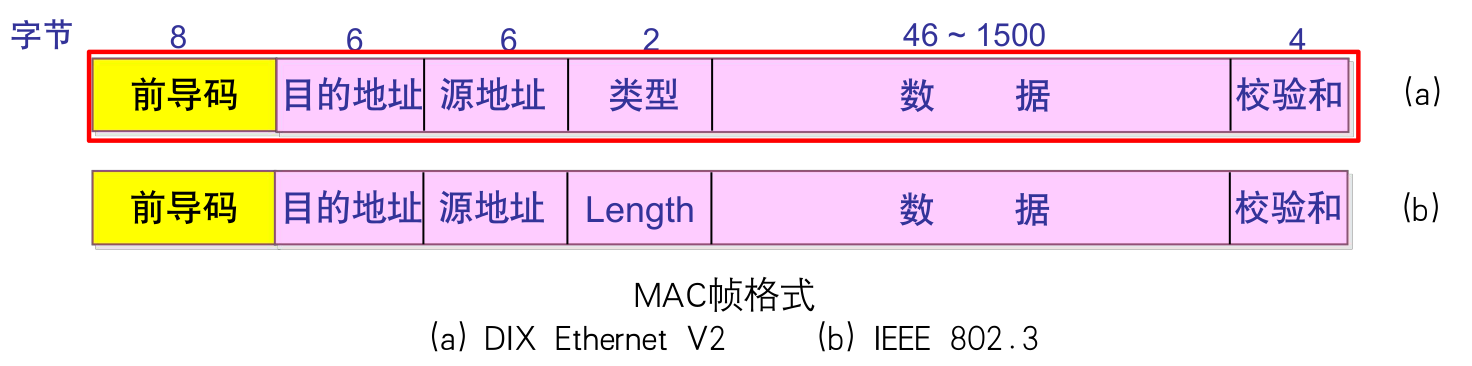
\includegraphics[width=0.95\textwidth]{ch03-ethernet-frame.png}
 \caption{Ethernet II 与 IEEE 802.3 帧的 2 B 字段分别表示 Type 和 Length；前导码通常不计入 MAC 帧长。来源：\texttt{Chapter3-数据链路层.pdf}，PDF 第 104 页（显示页 104），局部截取。}
 \label{fig:ch03-ethernet-frame}
\end{figure}

\annotationarea{4}

\subsection{以太网速率和物理层演进}
不同以太网标准通常保持 MAC 协议和基本帧格式，主要改变速率、物理介质和编码。课件列举 10 Mb/s、100 Mb/s、1 Gb/s、10 Gb/s、40/100 Gb/s 及更高速率，并比较光纤、铜缆和不同编码。

\begin{itemize}
 \item \textbf{快速以太网 100BASE-T：}速率为 100 Mb/s；BASE 表示基带传输，T 表示双绞线介质。
 \item \textbf{千兆以太网：}由 100 Mb/s 发展到 1 Gb/s，保留原有帧格式和基本工作方式。半双工模式为兼容可使用 CSMA/CD、载波扩充和帧突发；默认的全双工模式不使用 CSMA/CD。
 \item \textbf{万兆以太网：}10 Gb/s，只支持全双工，不使用 CSMA/CD，课件强调其改进重点在高速物理层。
 \item \textbf{40/100 Gb/s 及后续速率：}课件指出这些规范保留以太网帧格式和最小、最大帧长，并可通过可插拔模块适配不同物理介质。
\end{itemize}

课件第 107--108 页列出典型物理层方案，便于区分介质、速率和编码。UTP 指非屏蔽双绞线（Unshielded Twisted Pair）：
\begin{center}
\begin{tabularx}{0.98\textwidth}{l X l l}
\toprule
方案 & 介质与最大距离 & 编码（课件列值） & 速率\\
\midrule
1000BASE-SX & 多模光纤，约 550 m & 8B/10B & 1 Gb/s\\
1000BASE-LX & 光纤，约 5000 m & 8B/10B & 1 Gb/s\\
1000BASE-CX & 屏蔽双绞线，约 25 m & 8B/10B & 1 Gb/s\\
1000BASE-T & UTP，约 100 m & 4D-PAM5 & 1 Gb/s\\
10GBASE-SR & 多模光纤，约 300 m & 64B/66B & 10 Gb/s\\
10GBASE-LR & 单模光纤，约 10 km & 64B/66B & 10 Gb/s\\
10GBASE-ER & 单模光纤，约 40 km & 64B/66B & 10 Gb/s\\
10GBASE-CX4 & 双轴铜缆，约 15 m & 8B/10B & 10 Gb/s\\
10GBASE-T & UTP，约 100 m & 64B/65B & 10 Gb/s\\
\bottomrule
\end{tabularx}
\end{center}
课件第 107 页将 1000BASE-T 写为“2 对 UTP”；这与 IEEE 802.3ab 对 1000BASE-T 的“4 对五类平衡铜缆”规定不符，应视为课件表格笔误，按四对理解（\href{https://standards.ieee.org/ieee/802.3ab/1086/}{IEEE 802.3ab-1999}）。

课件第 111--112 页还列出 25/50 Gb/s、200/400 Gb/s、800 Gb/s 以及当时对 1.6 Tb/s 的路线图预测。它们是课件所引用的技术发展时间线；预测性描述应按课件当时的表述理解，不与本章协议机制混为一谈。

\annotationarea{4}

\subsection{以太网交换机：自学习、过滤和转发}
\textbf{交换机（switch）}是数据链路层设备，通常存储并转发以太网帧，对主机透明且即插即用。交换机的\textbf{交换表}至少记录“MAC 地址、到达该主机的接口、时间戳”。它按 MAC 地址转发帧，而不是按 IP 前缀路由。

交换机收到帧后执行以下步骤：
\begin{enumerate}
 \item \textbf{学习源地址：}将帧的源 MAC 与帧进入的接口对应起来，刷新或新增交换表项。
 \item \textbf{查询目的地址：}若目的地址在表中且对应另一个接口，则只从该接口转发；若目的已知且位于帧进入的同一网段，则过滤该帧，不再送回。
 \item \textbf{未知目的泛洪：}若表中没有目的地址，将帧转发到除输入接口外的其他接口。此时帧仍保留原来的目的 MAC 地址；“泛洪”指交换机复制帧的转发方式，不表示帧变成了广播帧。
\end{enumerate}
交换表项随时间老化；收到源 MAC 从新接口进入的帧时，交换机会更新映射。

\textbf{课件例题（PDF p.118）。} 交换机 6 个端口连接 A、B、C、A'、B'、C'，初始交换表为空；A 从端口 1 发帧给 A'，A' 从端口 4 回复。

\textbf{解：}A 发帧进入端口 1，交换机先学习 $(A,1)$。目的 A' 尚未知，故向其他端口泛洪；其他主机按目的 MAC 检查后丢弃，A' 收到。A' 回复时交换机学习 $(A',4)$，并查到 A 位于端口 1，于是只向端口 1 选择性转发。此后表中至少有 $A\to1$ 和 $A'\to4$ 两项。

\annotationarea{4}

\begin{figure}[H]
 \centering
 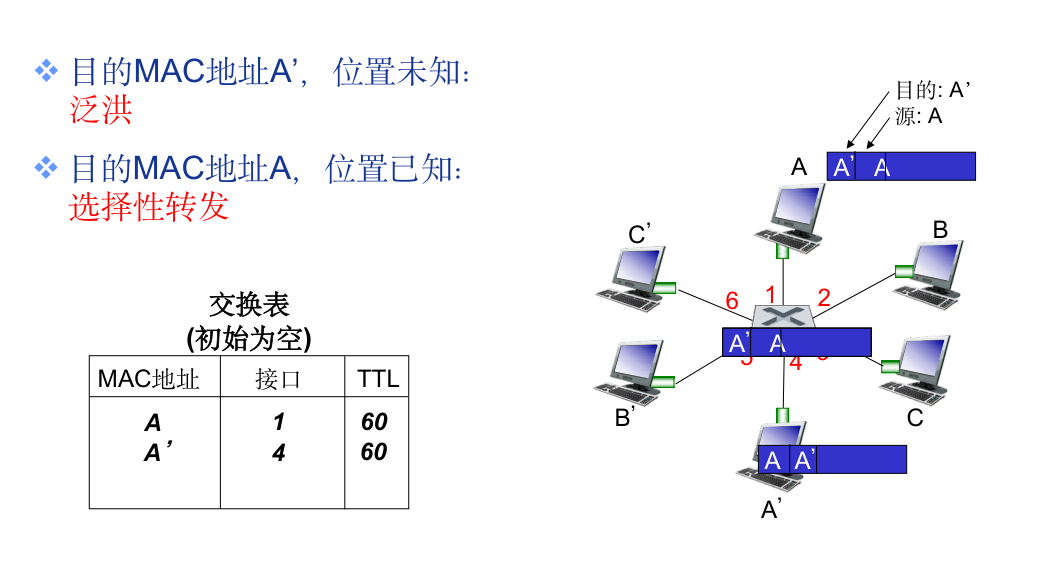
\includegraphics[width=0.86\textwidth]{ch03-switch-learning.png}
 \caption{首次目的地址未知时泛洪；交换机学习源地址后，返回帧可按表选择性转发。来源：\texttt{Chapter3-数据链路层.pdf}，PDF 第 118 页（显示页 118），局部截取。}
 \label{fig:ch03-switch-learning}
\end{figure}

\annotationarea{4}

\subsection{多交换机自学习例题}
\textbf{课件例题（PDF p.120）。} 拓扑中，交换机 $S_1$ 接主机 A、B、C 并连接 $S_4$；$S_2$ 接 D、E、F 并连接 $S_4$；$S_3$ 接 G、H、I 并连接 $S_4$。四台交换机的表初始为空。C 向 H 发帧，H 随后向 C 回应。求各交换机表项并说明转发过程。

\textbf{解：}
\begin{enumerate}
 \item C 的帧到 $S_1$。$S_1$ 学习 $C\to C$ 所连端口；H 未知，于是向 A、B、$S_4$ 方向泛洪。
 \item 帧到 $S_4$。$S_4$ 学习 $C\to S_1$；H 未知，向 $S_2$ 和 $S_3$ 方向泛洪。
 \item $S_2$、$S_3$ 分别学习 $C\to S_4$。两台交换机均未知 H，于是分别向本地终端端口泛洪；H 收到帧。
 \item H 回帧到 $S_3$。$S_3$ 学习 $H\to H$ 所连端口，查表知 C 在 $S_4$ 方向，只向 $S_4$ 转发。
 \item $S_4$ 学习 $H\to S_3$，查 C 在 $S_1$ 方向，只向 $S_1$ 转发。
 \item $S_1$ 学习 $H\to S_4$，查 C 在本地端口，只向 C 转发。$S_2$ 未收到回应帧，不会由该次通信学到 H。
\end{enumerate}

通信完成后，相关交换表至少含有：$S_1$：C 到本地 C 端口、H 到 $S_4$；$S_2$：C 到 $S_4$；$S_3$：C 到 $S_4$、H 到本地 H 端口；$S_4$：C 到 $S_1$、H 到 $S_3$。端口号按拓扑端口表示，没有从课件图中标出的端口编号处用相邻主机或交换机名称表示。

\annotationarea{4}

\subsection{Hub、交换机与冲突域}
\textbf{集线器（Hub）}工作在物理层，只再生或复制比特，不读取 MAC 地址。它不会隔离冲突域，也不会隔离广播域。\textbf{交换机和网桥}工作在数据链路层，能按帧地址过滤或转发，从而隔离冲突域，但普通二层交换机不会隔离广播域。路由器在网络层转发不同网络间的分组，通常构成广播域边界。

课件对设备的对照还列出即插即用、优化路由和直通传输：Hub、交换机、网桥均标为即插即用，不负责优化路由；直通传输是读出目的地址后即可开始转发，不等待完整帧到齐。采用存储转发时，交换机先接收完整帧并检查 FCS，再作转发决定。交换机端口专用、全双工时可支持多对端口并行通信；连接共享式 Hub 的端口仍按共享段规则工作。

\annotationarea{4}

\subsection{VLAN 与 IEEE 802.1Q}
单一大型广播域中的地址解析协议（Address Resolution Protocol，ARP）、动态主机配置协议（Dynamic Host Configuration Protocol，DHCP）和未知目的帧会到达较多链路，也带来管理、效率、隐私和隔离问题。\textbf{虚拟局域网（Virtual Local Area Network，VLAN）}将一个物理交换网络划分成多个逻辑广播域。主机更换物理位置后，若希望逻辑上仍属于原部门，可以通过 VLAN 成员配置保持其逻辑归属。

课件列出基于端口、MAC 地址、协议和子网的 VLAN 划分方法。端口 VLAN 最直观：把若干交换机端口分到同一 VLAN；端口可以按管理配置动态分配。不同 VLAN 之间不能直接进行二层通信；需要通过路由器或具有三层转发功能的交换机转发。

同一 VLAN 若跨越多台交换机，交换机之间的\textbf{中继端口（trunk port）}可以承载多个 VLAN 的帧。接入端口按本地配置识别 VLAN；帧通过 trunk 时需携带 VLAN 标识。

\textbf{IEEE 802.1Q}在以太网帧的源地址字段之后、类型字段之前插入 4 B VLAN 标记。其前 2 B 是标记协议标识符，值为 \texttt{0x8100}；后 2 B 的标记控制信息含 3 bit 优先级、1 bit 规范格式指示符（Canonical Format Indicator，CFI）和 12 bit VLAN 标识符（VLAN Identifier，VID）。VID 标识该帧所属的 VLAN。无标记帧为普通以太网帧；带标记帧用于交换机间携带 VLAN 信息。标签插入后 FCS 应按新帧内容计算。

\textbf{跨交换机转发例：}主机接入端口属于 VLAN 10，向另一台交换机上的 VLAN 10 主机发送帧。入口交换机按端口配置识别 VLAN 10，在 trunk 发出时插入 VID=10；出口交换机据 VID 只在 VLAN 10 内转发，并在向普通未标记接入口送出时去掉标签。VLAN 20 的端口不接收该帧。课件显示的最大数据载荷为 1500 B，插入 4 B 标记后最大帧长由 1518 B 增至 1522 B。

\begin{figure}[H]
 \centering
 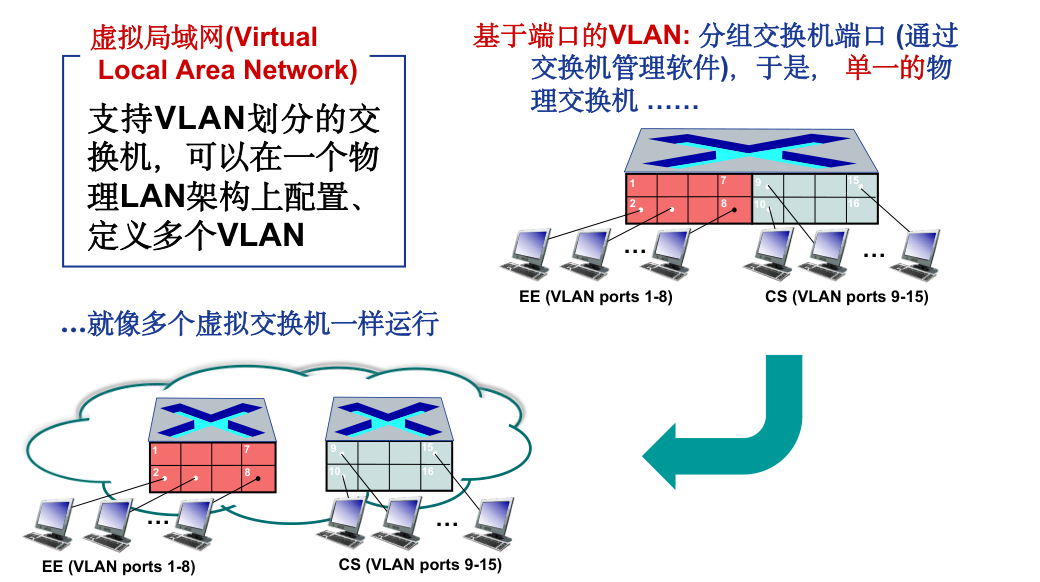
\includegraphics[width=0.86\textwidth]{ch03-vlan.png}
 \caption{同一物理交换网络被配置为多个逻辑 VLAN；广播只在相应 VLAN 内传播。来源：\texttt{Chapter3-数据链路层.pdf}，PDF 第 127 页（显示页 127），局部截取。}
 \label{fig:ch03-vlan}
\end{figure}

\annotationarea{4}

\begin{quote}\small 来源：课件 PDF 第 96--131 页（显示页 96--131）；参考书 §3.6，PDF 第 98--123 页（印刷第 87--112 页）及 §3.8，PDF 第 128--136 页（印刷第 117--125 页）。课件例题：交换机自学习第 118 页、多交换机转发第 120 页。课件第 105 页的 512 $\mu$s 与其 512 bit / 10 Mb/s 不一致，按计算结果订正为 51.2 $\mu$s。\end{quote}

\section{PPP 协议}

\subsection{点对点链路和 PPP 的设计需求}
\textbf{点对点链路}只有一个发送端和一个接收端，例如拨号或专线连接；与广播链路相比，不需要多个结点竞争信道，也不需要使用 MAC 地址从多个接收者中选择目的接口。课件列出高级数据链路控制（High-Level Data Link Control，HDLC）和点对点协议（Point-to-Point Protocol，PPP）两种点对点数据链路控制协议，本节重点讲 PPP。

\textbf{点对点协议（PPP，Point-to-Point Protocol）}由互联网工程任务组（Internet Engineering Task Force，IETF）制定，可在不同链路上运行，也可承载不同网络层协议。PPP 的设计需求包括：组帧并支持多种网络层载荷；对任意比特模式提供透明传输；检测差错；检测连接是否仍然活动并向网络层报告链路状态；协商网络层地址或相关配置。

PPP 不需支持差错纠正与恢复、流量控制、乱序交付或多点链路。差错恢复等功能可由高层协议处理。PPP 对帧作差错检测，但在数据传输期间不使用逐帧序号和 ACK 来恢复错误帧；因此，链路建立阶段存在控制协商，不代表每个数据帧均可靠交付。

\annotationarea{4}

\subsection{PPP 帧字段}
常见 PPP 帧由首尾标志字段、地址、控制、协议、信息和 FCS 组成。课件图示的常见未压缩格式为：
\begin{center}
\begin{tabularx}{0.98\textwidth}{l l X}
\toprule
字段 & 常见长度与值 & 作用\\
\midrule
Flag & 1 B，\texttt{0x7E} & 帧定界符，首尾各一个\\
Address & 1 B，\texttt{0xFF} & PPP 常见固定值，不是以太网目的 MAC\\
Control & 1 B，\texttt{0x03} & PPP 常见固定值\\
Protocol & 2 B & 标识信息字段的上层协议或控制协议\\
Information & 0--1500 B & 网络层数据报或 PPP 控制报文\\
FCS & 通常 2 B，也可为 4 B & CRC 差错检测字段\\
Flag & 1 B，\texttt{0x7E} & 帧结束定界符\\
\bottomrule
\end{tabularx}
\end{center}
课件把 Address、Control 描述为无效或暂未定义的字段。PPP 是点对点链路，不依靠它们作多站地址选择。PPP 不用 CSMA/CD，不需要以太网的 64 B 最小帧限制。

\begin{figure}[H]
 \centering
 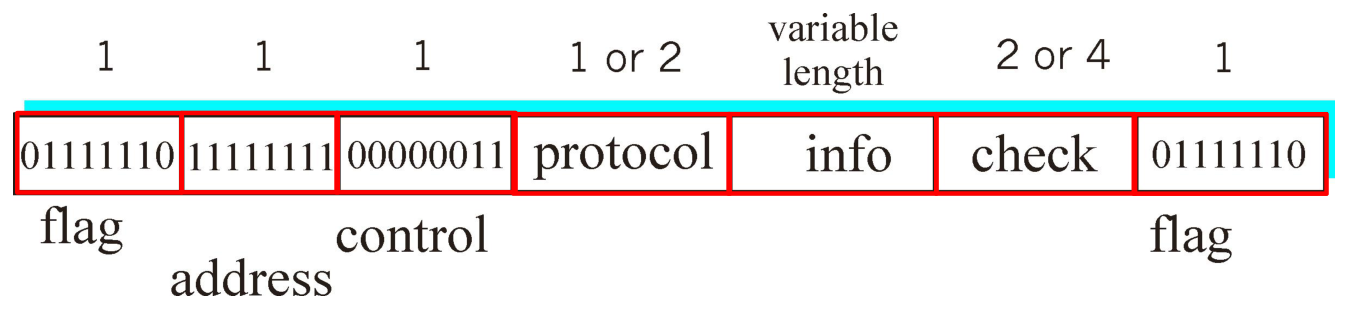
\includegraphics[width=0.94\textwidth]{ch03-ppp-frame-detail.png}
 \caption{PPP 帧字段及常见长度；Protocol 字段说明信息字段的协议类型。来源：\texttt{Chapter3-数据链路层.pdf}，PDF 第 137 页（显示页 137），局部截取。}
 \label{fig:ch03-ppp-frame}
\end{figure}

\annotationarea{4}

\subsection{PPP 的字节填充和零比特填充}
帧首尾使用 \texttt{0x7E} 定界，信息字段仍可能包含相同模式。PPP 按链路传输方式选择填充方法。

\textbf{异步传输：字节填充。} 转义字节为 \texttt{0x7D}。信息字段中的 \texttt{0x7E} 转为 \texttt{0x7D 0x5E}，\texttt{0x7D} 转为 \texttt{0x7D 0x5D}；原字节值和 \texttt{0x20} 做异或。数值小于 \texttt{0x20} 的控制字符也按规则转义，例如 \texttt{0x03} 变为 \texttt{0x7D 0x23}，\texttt{0x11} 变为 \texttt{0x7D 0x31}，\texttt{0x13} 变为 \texttt{0x7D 0x33}；课件还列出奇偶位为 1 的 \texttt{0x91} 和 \texttt{0x93}，分别变为 \texttt{0x7D 0xB1}、\texttt{0x7D 0xB3}。接收端去掉转义字节，并对转义后的值再次与 \texttt{0x20} 异或，恢复原字节。

\textbf{同步传输：零比特填充。} 帧内每连续出现 5 个 1 后插入 0；接收端删除连续 5 个 1 后的填充 0。该规则确保帧内数据不会冒充边界 \texttt{01111110}。

\annotationarea{4}

\subsection{LCP、认证、NCP 与 PPPoE}
在交换网络层数据前，两端需配置 PPP 链路并取得网络层所需信息。链路控制协议（Link Control Protocol，LCP）用于建立、配置和检测链路，也可协商最大帧长、认证等选项；若配置了认证，认证成功或双方不要求认证后继续；网络控制协议（Network Control Protocol，NCP）再配置所承载网络层协议的信息，例如 IP 地址。

课件第 141 页提到 IP 控制协议（IP Control Protocol，IPCP）报文用于配置 IP 信息，并把数值 8021 写成“IP 分组首部的上层协议字段”。这里应归属于\textbf{PPP 帧的 Protocol 字段}，且是十六进制 \texttt{0x8021}。参考书列出的常见值为：\texttt{0xC021} 表示 LCP，\texttt{0x8021} 表示 IPCP，\texttt{0x0021} 表示 IPv4 数据报。IPCP 与 IPv4 数据报因此不是同一类载荷。

\textbf{PPPoE（PPP over Ethernet）}把 PPP 会话承载在以太网链路上，常见于宽带接入。课件给出两种组网方式：机构网关作为一个 PPPoE 客户端，内部主机共享一个 PPP 会话；或者每台主机分别运行客户端，与运营商接入服务器各自建立会话。

课件将 PPPoE 工作过程分为三阶段：\textbf{Discovery} 获取对端以太网地址并确定会话 ID；\textbf{Session} 进行 PPP 协商并传输 PPP 数据；\textbf{Terminate} 发送报文结束会话。课件第 143 页将认证、加密和压缩并列为 PPPoE 能力；参考书对应内容主要说明 PPP 可协商认证、进行访问控制和计费。本笔记保留课件的接入场景，同时不把加密视为 PPP 帧或会话本身自动提供的属性。

\annotationarea{4}

\begin{quote}\small 来源：课件 PDF 第 132--146 页（显示页 132--146）；参考书 §3.7.2，PDF 第 125--126 页（印刷第 114--115 页）。课件第 141 页将 IPCP 的 \texttt{0x8021} 误称为 IP 首部字段；应为 PPP Protocol 字段。\end{quote}

\section{链路虚拟化}

\subsection{用 IP 屏蔽底层网络差异}
\textbf{虚拟化}是一种抽象方法：上层使用下层提供的统一接口，不必了解下层内部的每一个实现细节。课件用虚拟内存、虚拟设备等说明这种抽象，再将其用于网络。

互联网形成早期，不同网络有各自的寻址约定、分组格式、差错恢复和路由方法。课件列出的异构网络包括 ARPANET、电缆数据网络、ALOHA 卫星网络和分组无线网络。\par
IP 作为统一的网际层，为这些网络提供统一的网络层寻址和分组格式，使网络在网际层看起来较为一致；体系结构因此包含网际层地址和本地网络地址两层寻址。课件中的\textbf{网关（gateway）}把网际层分组封装进本地网络的分组格式，或从本地分组中取出网际层分组，再沿网际层路由到下一网关。

底层电缆、卫星、电话调制解调器等网络技术由各自的链路机制实现；异步传输模式（Asynchronous Transfer Mode，ATM）和多协议标签交换（Multiprotocol Label Switching，MPLS）等网络从 IP 路由器的视角可表现为连接两个 IP 路由器的逻辑链路。统一的 IP 层并不意味着底层网络使用相同帧格式或相同物理介质，而是通过逐层封装和接口抽象隐藏差异。

\begin{quote}\small 来源：\texttt{Chapter3-数据链路层.pdf}，PDF 第 147--152 页（显示页 147--152）。课件以 Cerf 与 Kahn 的互联网体系结构说明不同底层网络如何由统一的网际层连接；参考书第 3 章未设置完全对应的小节。\end{quote}
\annotationarea{2}
